%!TEX root = ../template.tex
%%%%%%%%%%%%%%%%%%%%%%%%%%%%%%%%%%%%%%%%%%%%%%%%%%%%%%%%%%%%%%%%%%%%
%% chapter2.tex
%% NOVA thesis document file
%%
%% Chapter with the template manual
%%%%%%%%%%%%%%%%%%%%%%%%%%%%%%%%%%%%%%%%%%%%%%%%%%%%%%%%%%%%%%%%%%%%

\typeout{NT FILE demmon.tex}

\chapter{DeMMON}
\label{cha:demmon}
% Define tab size for indentation
\algrenewcommand\algorithmicindent{2em}%

%%%%%%%%%%%%%%%%%%%%%%%%%%%%%%%%%%%%%%%%%%%%%%%%%%%%%%%%%%%%%%%%
% BLOCKS - \block[]
%%%%%%%%%%%%%%%%%%%%%%%%%%%%%%%%%%%%%%%%%%%%%%%%%%%%%%%%%%%%%%%%

% State, like all blocks ends with \asdend
\algblockdefx[asdstate]{asdstate}{asdend}
{\textbf{State}}{}


% Init
\algblockdefx[asdinit]{asdinit}{asdend}
{\textbf{Init}}{}

\algblockdefx[asdtypes]{asdtypes}{asdend}
{\textbf{Types}}{}

\algdef{SE}[SUBALG]{Indent}{EndIndent}{}{\algorithmicend\ }%
\algtext*{Indent}
\algtext*{EndIndent}

% Upon
\algblockdefx[asdupon]{asdupon}{asdend}
[1][Unknown]{\textbf{Upon} #1 \textbf{Do}}{}
\algblockdefx[asdupontimer]{asdupontimer}{asdend}
[1][Unknown]{\textbf{Upon Timer} #1 \textbf{Do}}{}

% For
\algblockdefx[asdfor]{asdfor}{asdend}
[1][Unknown]{\textbf{Forall} #1 \textbf{Do}}{}

\algblockdefx[asdrepeateveryx]{asdrepeateveryx}{asdend}
[1]{\textbf{Every} #1 \textbf{Do}}{}

% If
\algblockdefx[asdif]{asdif}{asdend}
[1][Unknown]{\textbf{If} (#1) \textbf{Then}}{}

% Else for If
\algcblockdefx[asdelsea]{asdif}{asdelsea}{asdend}
{\textbf{Else}}{}

% Else for Else If
\algcblockdefx[asdelseb]{asdelseif}{asdelseb}{asdend}
{\textbf{Else}}{}

% Else If
\algcblockdefx[asdelseif]{asdif}{asdelseif}{asdend}
[1][Unknown]{\textbf{Else If} (#1) \textbf{Then}}{}

% Interface
\algblockdefx[asdinterface]{asdinterface}{asdend}
{\textbf{Interface}}{}

% Requests
\algblockdefx[asdrequests]{asdrequests}{asdend}
{\textbf{Requests}}{}

% Indications
\algblockdefx[asdindications]{asdindications}{asdend}
{\textbf{Indications}}{}

% Procedure
\algblockdefx[asdprocedure]{asdprocedure}{asdend}
[1][Unknown]{\textbf{Procedure} #1}{}

% Forever
\algblockdefx[asdforever]{asdforever}{asdend}
{\textbf{Forever Do}}{}

%%%%%%%%%%%%%%%%%%%%%%%%%%%%%%%%%%%%%%%%%%%%%%%%%%%%%%%%%%%%%%%%
% STATEMENTS - \statement{} or \statement{}{}
%%%%%%%%%%%%%%%%%%%%%%%%%%%%%%%%%%%%%%%%%%%%%%%%%%%%%%%%%%%%%%%%

% Simple Statements
\newcommand{\asdstatement}[1]{\statenew{#1}}
\newcommand{\asdstatementbold}[1]{\statenew{\textbf{#1}}}

% Trigger
\newcommand{\asdtrigger}[1]{\statenew{\textbf{Trigger} #1}}

% Timer
\newcommand{\asdsetuptimer}[1]{\statenew{\textbf{Setup Timer} #1}}
\newcommand{\asdsetupptimer}[1]{\statenew{\textbf{Setup Periodic Timer} #1}}
\newcommand{\asdcanceltimer}[1]{\statenew{\textbf{Cancel Timer} #1}}

% Call
\newcommand{\asdcall}[1]{\statenew{\textbf{Call} #1}}

% Return - use [] due to xparse
\NewDocumentCommand{\asdreturn}{o}{
	\statenew{\textbf{Return}\IfValueT{#1}{ #1}}
}

% Comment (inline)
\makeatletter
\newcommand{\asdcomment}[1]{
	\parbox[t]{\dimexpr\linewidth-\ALG@thistlm-8em}{
		\strut
		//\space #1
		\strut
	}
}
\makeatother


% Comment (entire line)
\makeatletter
\newcommand{\asdlinecomment}[1]{
		\State \parbox[]{\dimexpr\textwidth-\leftmargin-\labelsep-\labelwidth}{
			//\space #1
		\strut}
}
\makeatother


%%%%%%%%%%%%%%%%%%%%%%%%%%%%%%%%%%%%%%%%%%%%%%%%%%%%%%%%%%%%%%%%
% VALUES
%%%%%%%%%%%%%%%%%%%%%%%%%%%%%%%%%%%%%%%%%%%%%%%%%%%%%%%%%%%%%%%%

% Booleans
\newcommand{\asdfalse}[0]{$false$}
\newcommand{\asdtrue}[0]{$true$}

% Map
\newcommand{\asdmap}[2]{#1{[}#2{]}}

% Set 
\newcommand{\asdset}[1]{$\{$#1$\}$}

%%%%%%%%%%%%%%%%%%%%%%%%%%%%%%%%%%%%%%%%%%%%%%%%%%%%%%%%%%%%%%%%
% Algebraic
%%%%%%%%%%%%%%%%%%%%%%%%%%%%%%%%%%%%%%%%%%%%%%%%%%%%%%%%%%%%%%%%

% Equals (assignment)
\newcommand{\asdassign}[0]{ $\longleftarrow$ }

\algblockdefx[Foreach]{Foreach}{EndForeach}[1]{\For{\textbf{each} #1}}{}

% Equals (comparison)
\newcommand{\asdeq}[2]{#1 $=$ #2}

% Not equals
\newcommand{\asdneq}[2]{#1 $\neq$ #2}

% Exists
\newcommand{\asdexists}[1]{$\exists$ #1}

% Not Exists
\newcommand{\asdnexists}[1]{$\nexists$ #1}

% And
\newcommand{\asdand}[2]{#1 $\wedge$ #2}

% Or
\newcommand{\asdor}[2]{#1 $\vee$ #2}

% Except
\newcommand{\asdexcept}[2]{#1 $\setminus$ #2}

% Union
\newcommand{\asdunion}[2]{#1 $\bigcup$ #2}

% Belongs to
\newcommand{\asdin}[2]{#1 $\in$ #2}

% Not belongs to
\newcommand{\asdnotin}[2]{#1 $\notin$ #2}

% Bottom
\newcommand{\asdbottom}{$ \perp $}

\algnewcommand{\IfThenElse}[3]{% \IfThenElse{<if>}{<then>}{<else>}
  \State \algorithmicif\ #1\ \algorithmicthen\ #2\ \State \algorithmicelse\ #3}


%%%%%%%%%%%%%%%%%%%%%%%%%%%%%%%%%%%%%%%%%%%%%%%%%%%%%%%%%%%%%%%%
% Other
%%%%%%%%%%%%%%%%%%%%%%%%%%%%%%%%%%%%%%%%%%%%%%%%%%%%%%%%%%%%%%%%

\newcommand{\asdnewline}{\hfill\State}

DeMMon (Decentralized Management and Monitoring Overlay Network) is an overlay network aiming to create logical connections among nodes integrating the network, forming multiple tree-shaped networks. Then, it provides an API to request information about nodes and services running in the system, which is collected on-demand by the monitoring protocol via efficient information aggregation and dissemination using the tree structure.

In this chapter, we will begin by explaining the targeted environment and the operation of the overlay network, whose tree shape is the basis for the aggregation protocol. After, detail how the aggregation protocol performs aggregations in the tree, and lastly, list the operations exposed by the API and discuss how it interacts with the remaining components. \todo{insert refs to subsections ahead}

This solution, as observable in Figure~\ref{fig:demmon-overview}, is composed of three major components:

\begin{figure}[htbp]
    \centering
    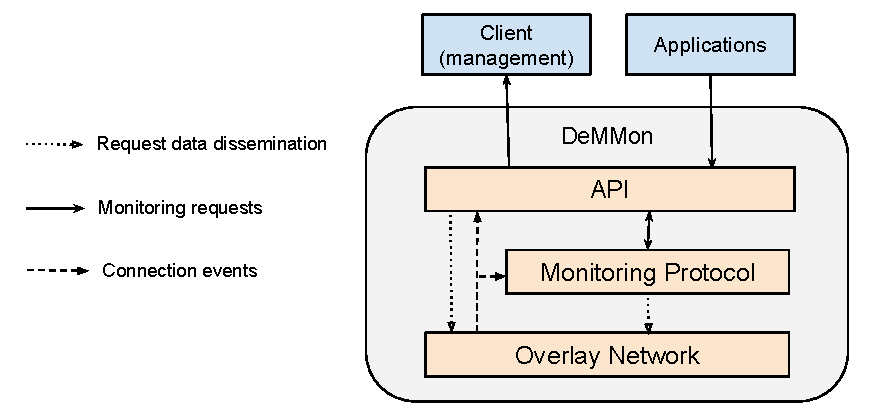
\includegraphics[width=\textwidth]{Chapters/Figures/DeMMon-arch-overview.pdf}
    \caption{An overview of the architecture of DeMMon}
    \label{fig:demmon-overview}
\end{figure}


\begin{enumerate}
    \item The overlay network, which strives to build the tree-shaped network, nodes in this network use latency, node capacity, and a set of logical rules to change their location in the tree.

    \item The monitoring protocol, which is a component that collects and disseminates information using the overlay network's established connections. It communicates via notifications and asynchronous request-replies with the overlay network to receive updates regarding established connections and connection failures. Lastly, it receives requests from the API to collect information.

    \item Lastly, the API receives updates from both the overlay network and the monitoring protocol, exposes the received information from those layers, and allows ingestion of new information. Furthermore, it allows issuing commands to collect new information, perform local aggregations periodically, or trigger issued alarms based on the respective conditions.
\end{enumerate}

\section{Overlay network}

In this section, we discuss the design of the overlay network, which aims to build and maintain a latency and capacity-aware tree-shaped network (capacity represents one, or a combination of, values that denote the node's computing and networking power). We begin by providing the considered system model, then follow with an overview of the mechanisms responsible for building and maintaining the tree. Lastly, we conclude the chapter with a summary and discussion of the protocol.

\subsection{System Model}

The assumed system model is assumed to be a distributed scenario composed of nodes connected to the internet set-up such that they can send and receive messages via the internet (with an external IP or port-forwarding). We also assume that nodes are spread throughout a large area and have varied capacity values.

Regarding the fault model, we assume that all but a small portion of nodes (also known as the landmarks, which in our model represent DCs) can fail, and when other nodes fail, they do so in a crash-fault manner, stopping all emissions and receptions of messages. We assume landmarks have additional fault tolerance given their privileged infrastructure, and additionally, we assume other such as replication~\cite{} mechanisms could be employed to ensure that faulty landmarks get replaced in case of failure. 

Finally, all nodes must run the same software stack with similar configuration settings and landmark values, installed a priori.

\subsection{Overview}

As previously mentioned, the main objective of the created protocol is to establish a latency and capacity-aware tree-shaped network. Our motivations for choosing the tree structure for the network are: (1) to be able to map the heterogeneity of each device in the environment: by biasing the placement of nodes in the tree such that nodes with higher capacity are placed higher in the tree, and nodes with lower capacity are biased towards lower levels of the tree, nodes are used more or less according to their capacity values; (2) the tree structure can be easily employed to perform efficient aggregations, by propagating and merging values recursively from the lower to the higher levels of the tree, which is the basis for the aggregation protocol presented in \todo{add ref}; and finally, (3) by leveraging on the tree structure, nodes can propagate information efficiently, given that, in a network composed of N nodes, broadcasts require only N-1 message transmissions to reach all nodes in the network. 

The devised membership protocol is coalesced by three main mechanisms: (1) the \textbf{join} mechanism, which aims to establish the initial tree structure, (2) the \textbf{active view maintenance}, responsible for bounding the number of connections for each node, and optimizing the connections of each node, (3)  and finally \textbf{passive view maintenance}, responsible for collecting information about peers which are not in the active view, which are used for both fault tolerance and connection optimizations.

\subsubsection{Join mechanism}

As previously mentioned, the join mechanism is the mechanism responsible for creating the initial tree structure. This mechanism is the first to be executed by all nodes in the system. Its first step (line~\ref{alg:state:state} of alg.~\ref{alg:state}) is to initialize the state of the joining node, composed by: (1) a map of type Node containing all successfully contacted nodes so far the join process, (2) a collection of type Node with all the nodes currently being contacted, (3) a set of timer ids for each node being contacted, (4) the best node contacted so far in the join process, (5) a timer id for contacting the chosen node in the join process, and finally (5) a variable of type Node denoting the peer itself. The type ``Node'' is a collection of attributes regarding a node, such as: latency measured, its parent, its number of children, among others.





This protocol varies largely depending on wether the joining node is a landmark or not. In case the joining node is a landmark, then it simply 

% JOIN -----

\begin{algorithm}
    % \setstretch{0.85}
\begin{algorithmic}[1]
    \caption{Join Protocol} \label{alg:memb:join}
    \asdtypes
        \State Node : <lat, parentIP, nrChildren, replied, IP, children<IP,  nrChildren>>
    \asdend
    \asdstate \label{alg:memb:join:state}
        \State contactedNodes \Comment{ collection of all successfully contacted nodes}
        \State nodesToContact \Comment{ nodes being contacted}
        \State landmarks \Comment{ landmark nodes}
        \State joinTimeouts \Comment{ collection of contacted nodes -> timerIDs}
        \State bestPeerLastLevel : Node \Comment{the best peer contacted so far in the join process}
        \State joinReqTimeoutTid \Comment{ timerID for join messages}
        \State self : Node \Comment{ myself}
    \asdend

\asdupon[Init(landmarks : IP[], selfIP, isLandmark)] \label{alg:memb:join:init}
    \State landmarks \asdassign landmarks 
    \State joinTimeouts, prevBestP \asdassign \{\}, nil
    \IfThenElse{isLandmark}
    {addLandmarkUntilSuccess(landmarks)} \label{alg:memb:join:add_land}
    {contactNodes(landmarks)} \label{alg:memb:join:contact_landm}
\asdend


\asdupon[receive(Join<>,sender)] \label{alg:memb:join:recv_join}
    \State sendMessageSideChannel(JoinReply<self.parent, self.node, self.children>, sender) 
\asdend
    
\asdupon[receive JoinReply(<parentIP, node, children>, sender) \&\& measuredLatency(lat)]  \label{alg:memb:join:recv_join_reply}
        \If{(\asdin{parentIP}{Landmarks} || \asdin{parentIP}{contactedNodes}) \&\& \asdin{node.IP}{nodesToContact}} 
            \State nodesToContact[node.IP].lat \asdassign lat
            \State nodesToContact[node.IP].children \asdassign children
            \State nodesToContact[node.IP].parent \asdassign parentIP
            \State nodesToContact[node.IP].replied \asdassign true
            \State cancelTimer(joinTimeouts[sender])
            \State delete(joinTimeouts, sender)
        \Else
            \State nodesToContact.delete(node)
        \EndIf
\asdend

\asdupon[(forall n $\in$ nodesToContact -> n.replied)]
    \State contactedNodes.appendAll(nodesToContact)
    \For{node in sortedByLatency(nodesToContact)}
        \If{(\asdnotin{node.IP}{landmarks}) \&\& node.nrChildren == 0} \label{alg:memb:join:verif_children}
            \State continue \Comment{check if node has enough children}
        \EndIf
        \If{prevBestP != nil \&\& (prevBestP.lat $\le$ node.lat || prevBestP.nrChildren < config.minGroupSize)} \label{alg:memb:join:verif_vs_prev}
            \State joinAsChild(prevBestP)
        \Else
            \State prevBestP \asdassign node \label{alg:memb:join:advance}
            \State toContact \asdassign [\asdin{c}{prevBestP.children} -> c.nrChildren >= config.minGroupSize]
            \State contactNodes([c.IP for c in toContact])
        \EndIf
        \State return
    \EndFor
    \IfThenElse{prevBestP != nil} 
    {joinAsChild(prevBestP)}  
    {abortJoinAndRetryLater()} \label{alg:memb:join:join_base_case}
    \State return
\asdend

\asdupon[JoinTimeoutTimer(node) || NodeMeasuringFailed(node)] \label{alg:memb:join:exclusions}
    \IfThenElse{(L in Landmarks)}{abortJoinAndRetryLater()}{delete(nodesToContact[L])} 
\asdend

\asdupon[JoinRequestTimer(p : Node)]
    \If {sender == prevBestP}
        \If{p.parentIP != nil}
            \State prevBestP \asdassign contactedNodes[p.parentIP]
            \State joinAsChild(prevBestP)
        \Else
            \State abortJoinAndRetryLater()
        \EndIf
    \EndIf
\asdend

\asdupon[receive(JoinRequest<>, sender)]
    \State addChildren(sender) \Comment{new chilren is established}
    \State sendMessageSideChannel(JoinRequestReply<generatedID,self,children>, p.IP)
\asdend
    
\asdupon[receive(JoinRequestReply<attributedId,parent,siblings>, sender)]
    \If {sender == prevBestP} 
        \State addParent(sender) \Comment{Adds Parent is established, join complete}
        \State cancelTimer(joinReqTimeoutTid)
    \EndIf
\asdend

\asdprocedure[joinAsChild(p : Node)]
    \State joinReqTimeoutTid \asdassign setupTimer(JoinRequestTimer<p>, config.JoinTimeout)
    \State sendMessageSideChannel(JoinRequest<>, p.IP)
\asdend

\asdprocedure[contactNodes(ips : IP[])]
    \State nodesToContact \asdassign \{\}
    \State toContact \asdassign [Node<0,nil,0,false,lIP,false,[]> for ip in ips]
    \For{n in toContact}
        \State nodesToContact[n] \asdassign n
        \State MeasureNode(n) 
        \State sendMessageSideChannel(JoinMessage<>, n)
        \State joinTimeouts[n] \asdassign \asdassign setupTimer(JoinTimeoutTimer(n), config.JoinTimeout)
    \EndFor
\asdend

\end{algorithmic}
\end{algorithm}


\begin{algorithm}
    % \setstretch{0.85}
    \begin{algorithmic}[1]

        \caption{Membership protocol (Active view Optimization)}

        \asdstate
        \State childrenLatencies : dict<string:dict<string:number>>
        \asdend

        \asdrepeateveryx{config.updateChildPeriodicity}
        \If{parent != nil}
        \State sLatencies = set()
        \For{sibling in siblings}
        \State sLatencies.append(<sibling.IP,sibling.measuredLatency)
        \EndFor
        \State sendMessage(UpdateChildStatus<children, siblingLatencies>, parent)
        \EndIf
        \asdend

        \asdrepeateveryx{config.updateParentPeriodicity}
        \For{child in chidren}
        \State sendMessage(UpdateParentStatus<self,child.ID, parent>)
        \EndFor
        \asdend

        \asdupon[receive(UpdateParentStatus<parent,myID, grandParent>, sender)]
        \If{sender == parent.IP}
        \State parent = parent
        \State self.ID = parent.ID + myID
        \State grandParent = grandParent
        \EndIf
        \asdend

        \asdupon[receive(UpdateChildStatus<child, childSiblingLatencies>, sender)]
        \If{children[sender] != nil}
        \State children[sender] = children
        \State childrenLatencies[sender]=childSiblingLatencies
        \EndIf
        \asdend

        \asdrepeateveryx{config.updateChildPeriodicity}
        \State childrenLatValues = set()
        \For{c1 in children}
        \For{<c2, lat> in childrenLatencies[c]}
        \If{lat - c1.measuredLatency >= d.config.maxLatDowngrade}
        \State break
        \EndIf
        \State higherBwC = c1
        \State lowerBWC = c2
        \If{c2.bw > c1.bw}
        \State higherBwC = c2
        \State lowerBWC = c1
        \EndIf
        \State childrenLatValues.add(<higherBwC,lowerBWC,lat>)
        \EndFor
        \EndFor
        \State kickedNodes = set()
        \State newParents = set()
        \State potentialChildren = dict<string,set<Node>>
        \State sortByLatency(childrenLatValues)

        \For{<higherBwC,lowerBWC,lat> in childrenLatValues}
        \If{len(children) - len(kickedNodes) <= config.MinGroupSize}
        \State break
        \EndIf
        \If{higherBwC in kickedNodes or lowerBWC in kickedNodes}
        \State continue
        \EndIf
        \If{loserBWC in newParents}
        \State continue
        \EndIf
        \If{higherBwNode.nrChildren == 0}
        \State potentialChildren[higherBwNode].append(lowerBWC)
        \If{len(potentialChildren) >= config.MinGroupSize}
        \For{potentialChild in potentialChildren[higherBwNode]}
        \State newParents <- newParents + higherBwNode
        \State send(OptimizationPropose<higherBwNode>, potentialChild)
        \State higherBwNode.nrChildren++
        \State kickedNodes <- kickedNodes + potentialChild
        \EndFor
        \For{<nIP,potentialChilren> in potentialChildren}
        \State potentialChilren.deleteAll(potentialChildren[higherBwNode])
        \EndFor
        \State potentialChildren[higherBwNode] = set<Node>
        \State continue
        \EndIf
        \EndIf
        \State kickedNodes <- kickedNodes + lowerBWC
        \State send(OptimizationPropose<higherBwNode>, lowerBWNode)
        \EndFor
        \asdend

        \asdupon[receive(OptimizationPropose<newParent>, sender)]
        \If{sender == parent}
        \State send(OptimizationProposeRequest<sender>, newParent)
        \EndIf
        \asdend

        \asdupon[receive(OptimizationProposeRequest<p>, sender)]
        \If{ p == parent \&\& sender in siblings} \Comment{ parent issuing the message is the same parent that i have}
        \State send(OptimizationProposeRequestReply<true>, sender)
        \Else
        \State sendSideChannel(OptimizationProposeRequestReply<false>, sender)
        \EndIf
        \asdend

        \asdupon[receive(OptimizationProposeRequestReply<reply>, sender)]
        \If{reply}
        \State sendMessageAndDisconnectFrom(DisconnectMessage<>, parent)
        \State addParent(sender)
        \EndIf
        \asdend

    \end{algorithmic}
\end{algorithm}

\begin{algorithm}
\begin{algorithmic}[1]

        \caption{Oportunistic Optimization}

    \asdstate
        \State childrenLatencies : dict<string:dict<string:number>>
    \asdend

    \asdrepeateveryx[config.OportunisticOptimizationTimeout]
        \State toMeasureRand = getRandSample(eView, config.NrPeersToMeasureRandom)
        \State toMeasureBiasedOpts = sortByEuclideanDist(eView / toMeasureRand)
        \State toMeasureBiased = getRandSample(toMeasureBiasedOpts, config.NrPeersToMeasureRandom)

        \For p in toMeasureRand:
            \State measurePeer(p)
        \EndFor
        \For p in toMeasureBiased:
            \State measurePeer(p)
        \EndFor
    \asdend

    \asdupon{peerMeasured(p, latency)}
        \State latencyImprovement := parent.measuredLatency - Latency
        \If{latencyImprovement >= config.MinLatencyForImprovement}:
            \State sendMessageSideChannel(OportunisticImprovementReq<self>,p)
        \EndIf
    \asdend


    \asdupon{receive(OportunisticImprovementReq<p>,sender)}
        \If{isDescendent(p.ID,self)}:
            \State sendMessageSideChannel(OportunisticImprovementReqReply<false>,sender)
        \Else
            \State addChildren(sender)
            \State sendMessageSideChannel(OportunisticImprovementReqReply<true>,sender)
        \EndIf
    \asdend

    \asdupon{receive(OportunisticImprovementReqReply<answer>,sender)}
        \If {answer} 
            \State addParent(sender)
        \EndIf
    \asdend

\end{algorithmic}
\end{algorithm}

\subsection{Summary}

\section{Monitoring protocol}

\subsection{Overview}

\subsection{Aggregation mechanisms}

\subsubsection{Single root aggregation}

\subsubsection{Multi root aggregation}

\subsubsection{Neighbourhood aggregation}

\subsection{Summary}

\section{API}

\subsection{System Model}

\subsection{Overview}

\subsection{Showcase}